\documentclass[11pt]{article}

\usepackage[margin=1in]{geometry}
\usepackage{fancyhdr}
\pagestyle{fancy}
\usepackage{amsmath}
\usepackage{amssymb}
\usepackage{graphicx}
\lhead{Chaitanya Pawa}
\chead{Statistical Data Mining II\ Homework 1}
\rhead{March 1, 2019}


\begin{document}

\begin{enumerate}
\item \textbf{Problem 1}
\\
In this exercise, we consider the MovieLense data in the “recommenderlab” package. The data set consisted of data from 943 users and 1664 movies. 
\\Firstly, we normalized the ratings to get a measure of how the ratings were distributed. The following two figures show how the normalized ratings of first 100 users are distributed and count of ratings per movie.
\begin{center}
    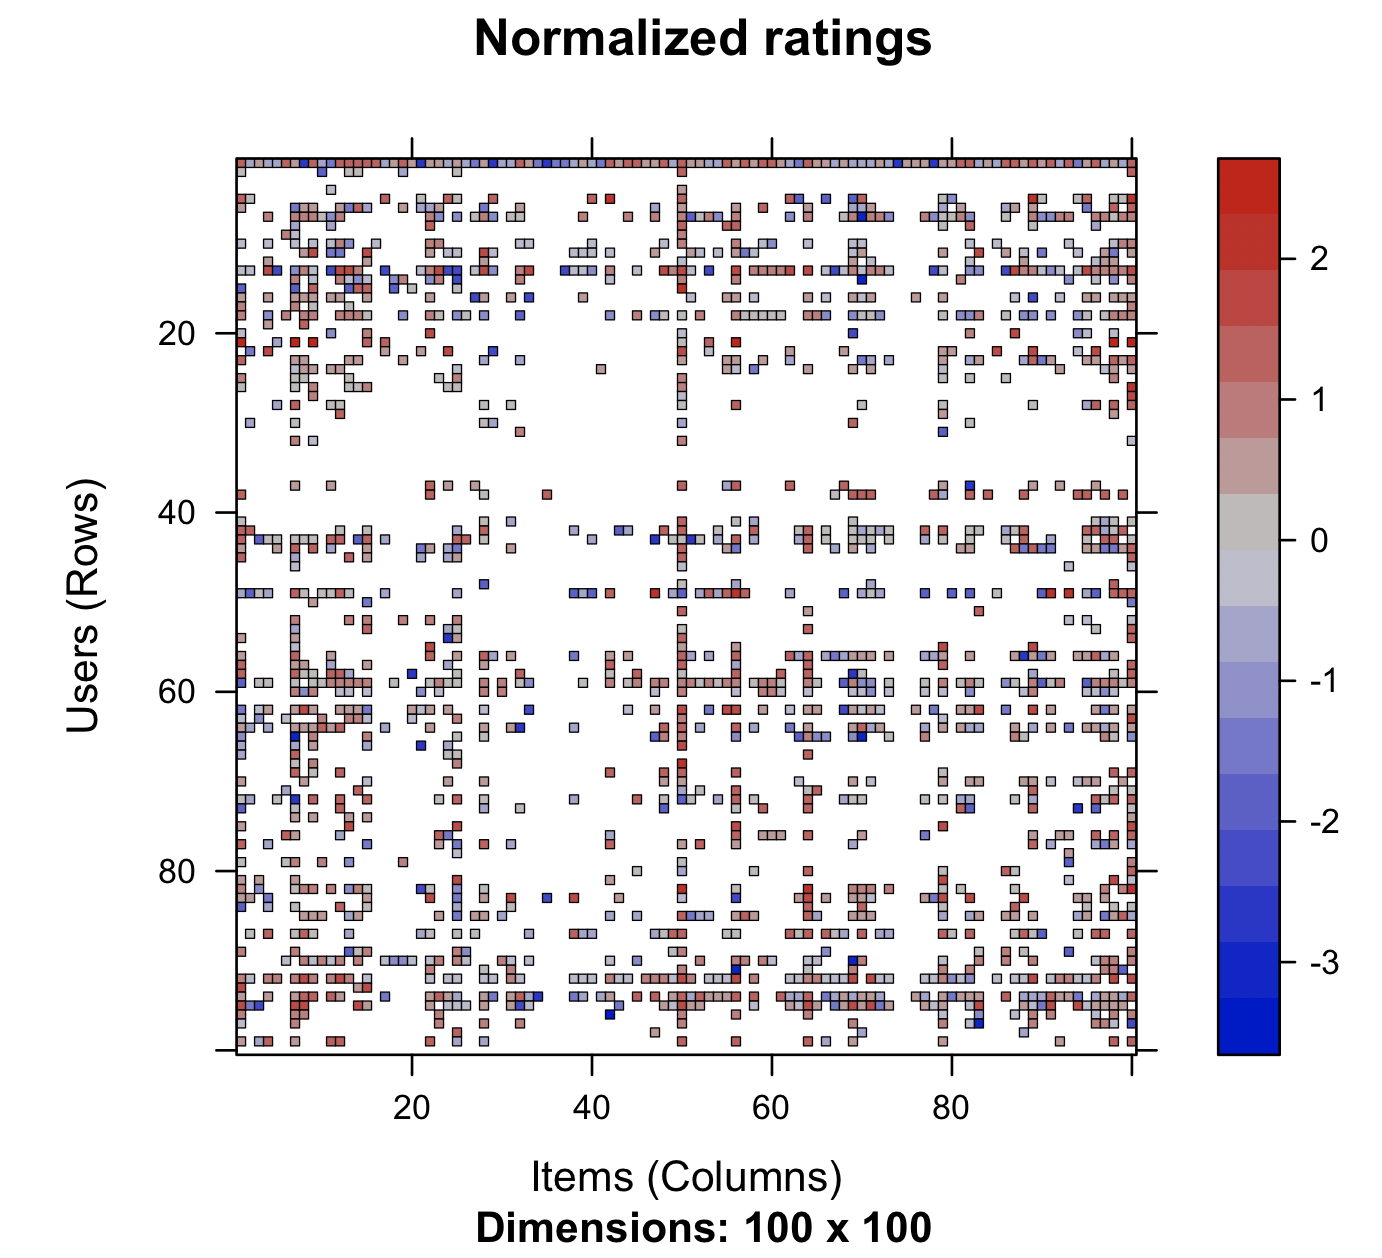
\includegraphics[height=0.4\textwidth]{klkl.png}
    \\\footnotesize Figure 1.1 : Normalized Rating Distribution
\end{center}
\begin{center}
    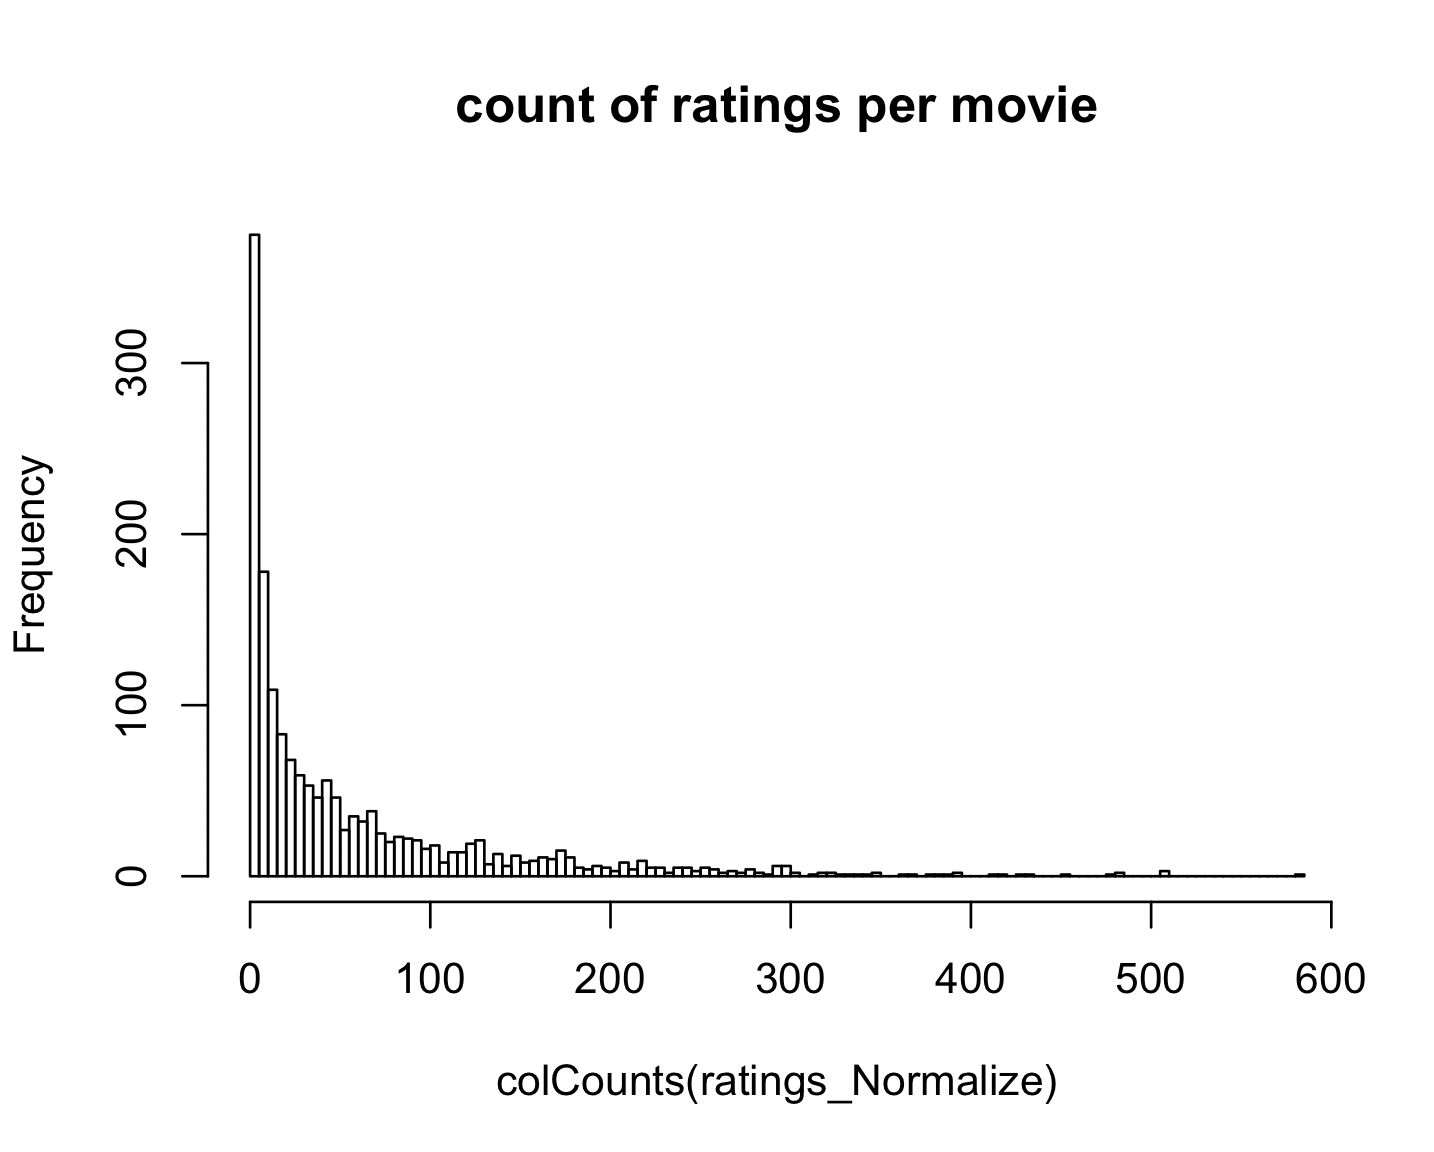
\includegraphics[height=0.4\textwidth]{klklkl.png}
    \\\footnotesize Figure 1.2 : Count of Ratings per Movie
\end{center}

\begin{enumerate}
    \item We designed our recommendation model where for each user “i” and each movie “j” they did not see, find top “k” most similar users to “i” who have seen “j” and then use them to infer the user “i” ’s rating on movie.
    \\We used this above model of User Based Collaborative filtering to predict the top 10 movie recommendations for each user. The data was then exported to "recom.RData" file. We also used the model to predict all the missing ratings in the original ratings matrix.
    \item We tested the performance of our system using cross-validation. We ran our algorithm 5 times. In each step, we used the training partition to make predictions for each user on all terms rated in the test partition (by that user). When we complete all 5 iterations, we will have a large number of user-movie pairs from the 5 test partitions on which you can evaluate the performance of your system. We then measured the performance of our recommendation system using evaluation scheme.
    \\For evaluation, we took the values of folds as 5, the value for given as 100 and took 60\% of the data as our training set. After evaluating, we got the following errors for the model.
    \begin{center}
    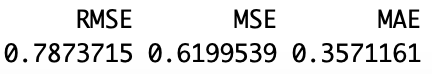
\includegraphics[width=0.4\textwidth]{dff.png}
    \\\footnotesize Figure 1.3 : ERRORS 
\end{center}
We then evaluated using cross-validation to check for the results with different values of n and thus find the most suitable value for it. For each value of n we got the following confusion matrix for the data.
\begin{center}
    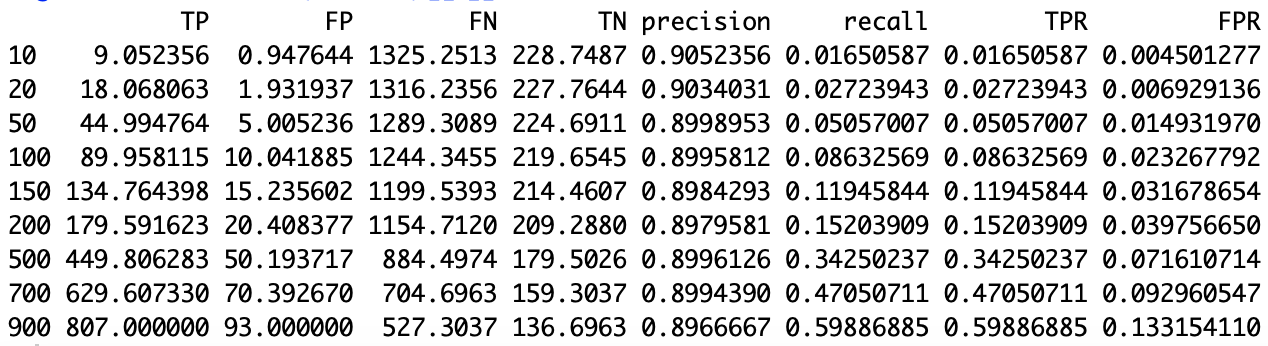
\includegraphics[width=0.8\textwidth]{tyui.png}
    \\\footnotesize Figure 1.4 : Confusion Matrix
\end{center}

We then tried to find the best value for n. We plotted two graphs, one for True Positive Rate vs False Positive Rate and the other for Precision vs Recall.
\begin{center}
    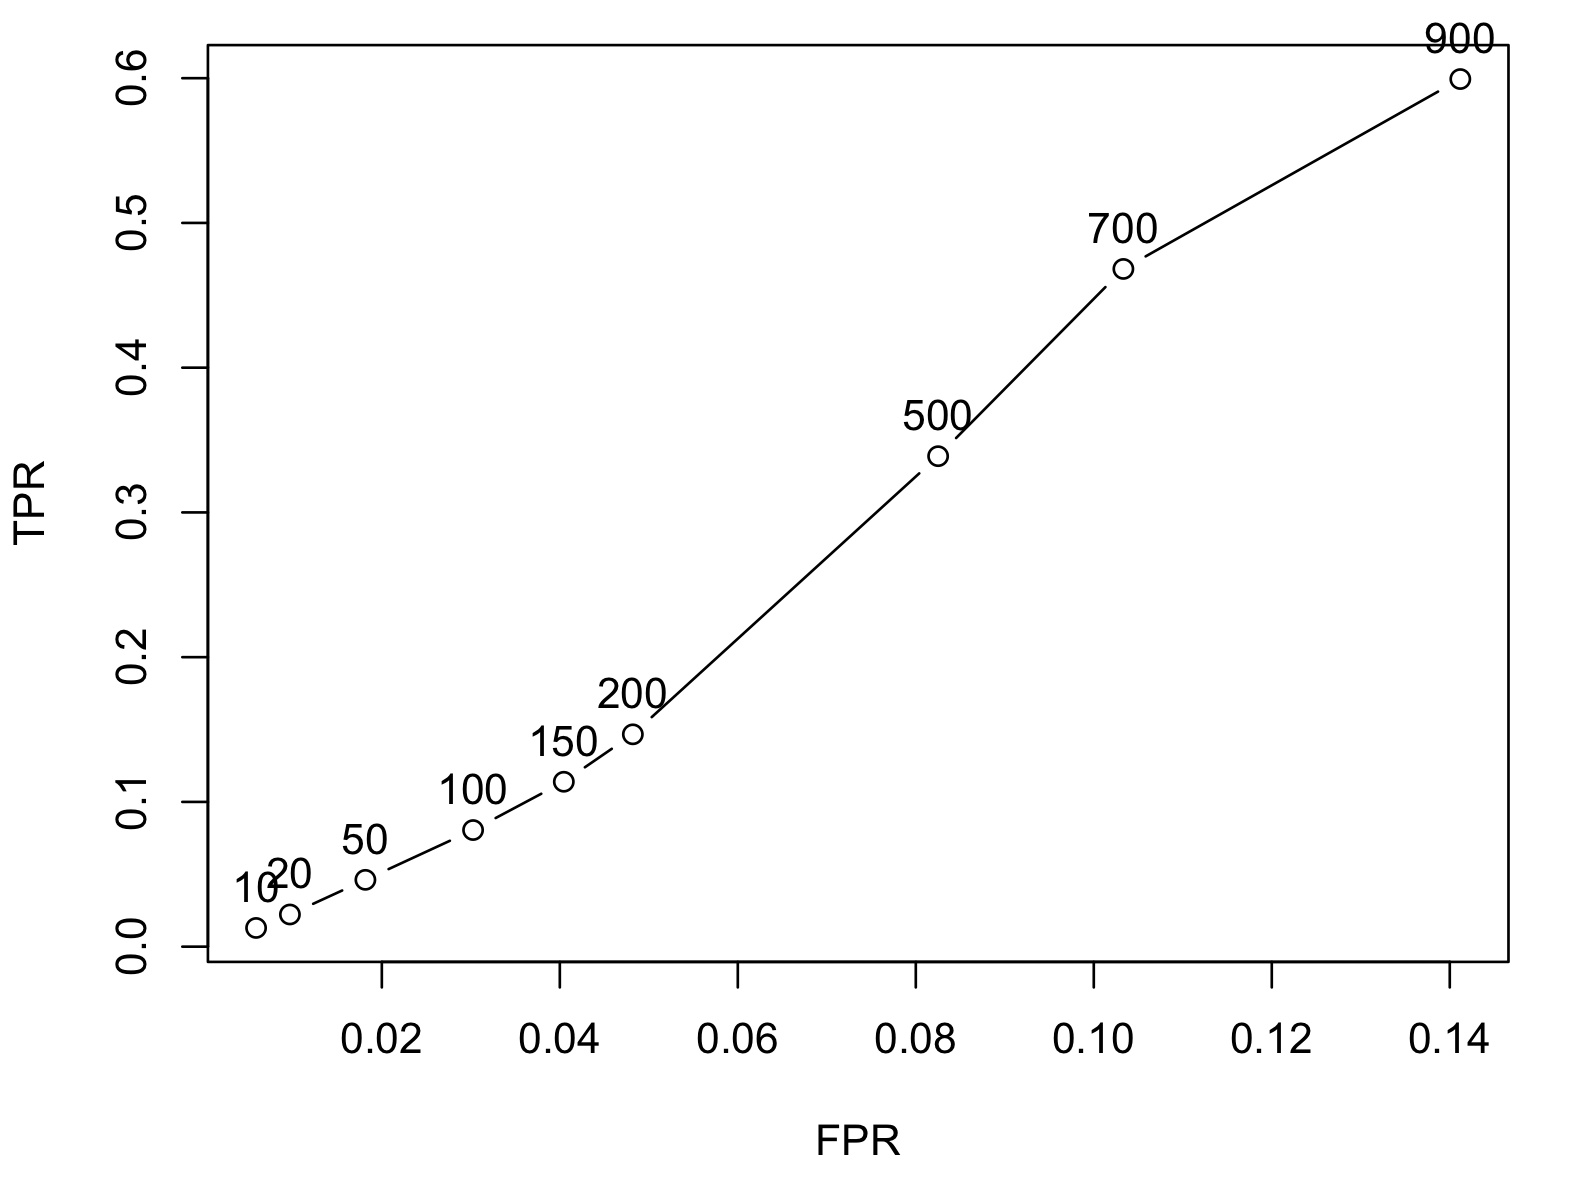
\includegraphics[width=0.6\textwidth]{gbhj.png}
    \\\footnotesize Figure 1.5 : TPR  vs FPR
\end{center}
\begin{center}
    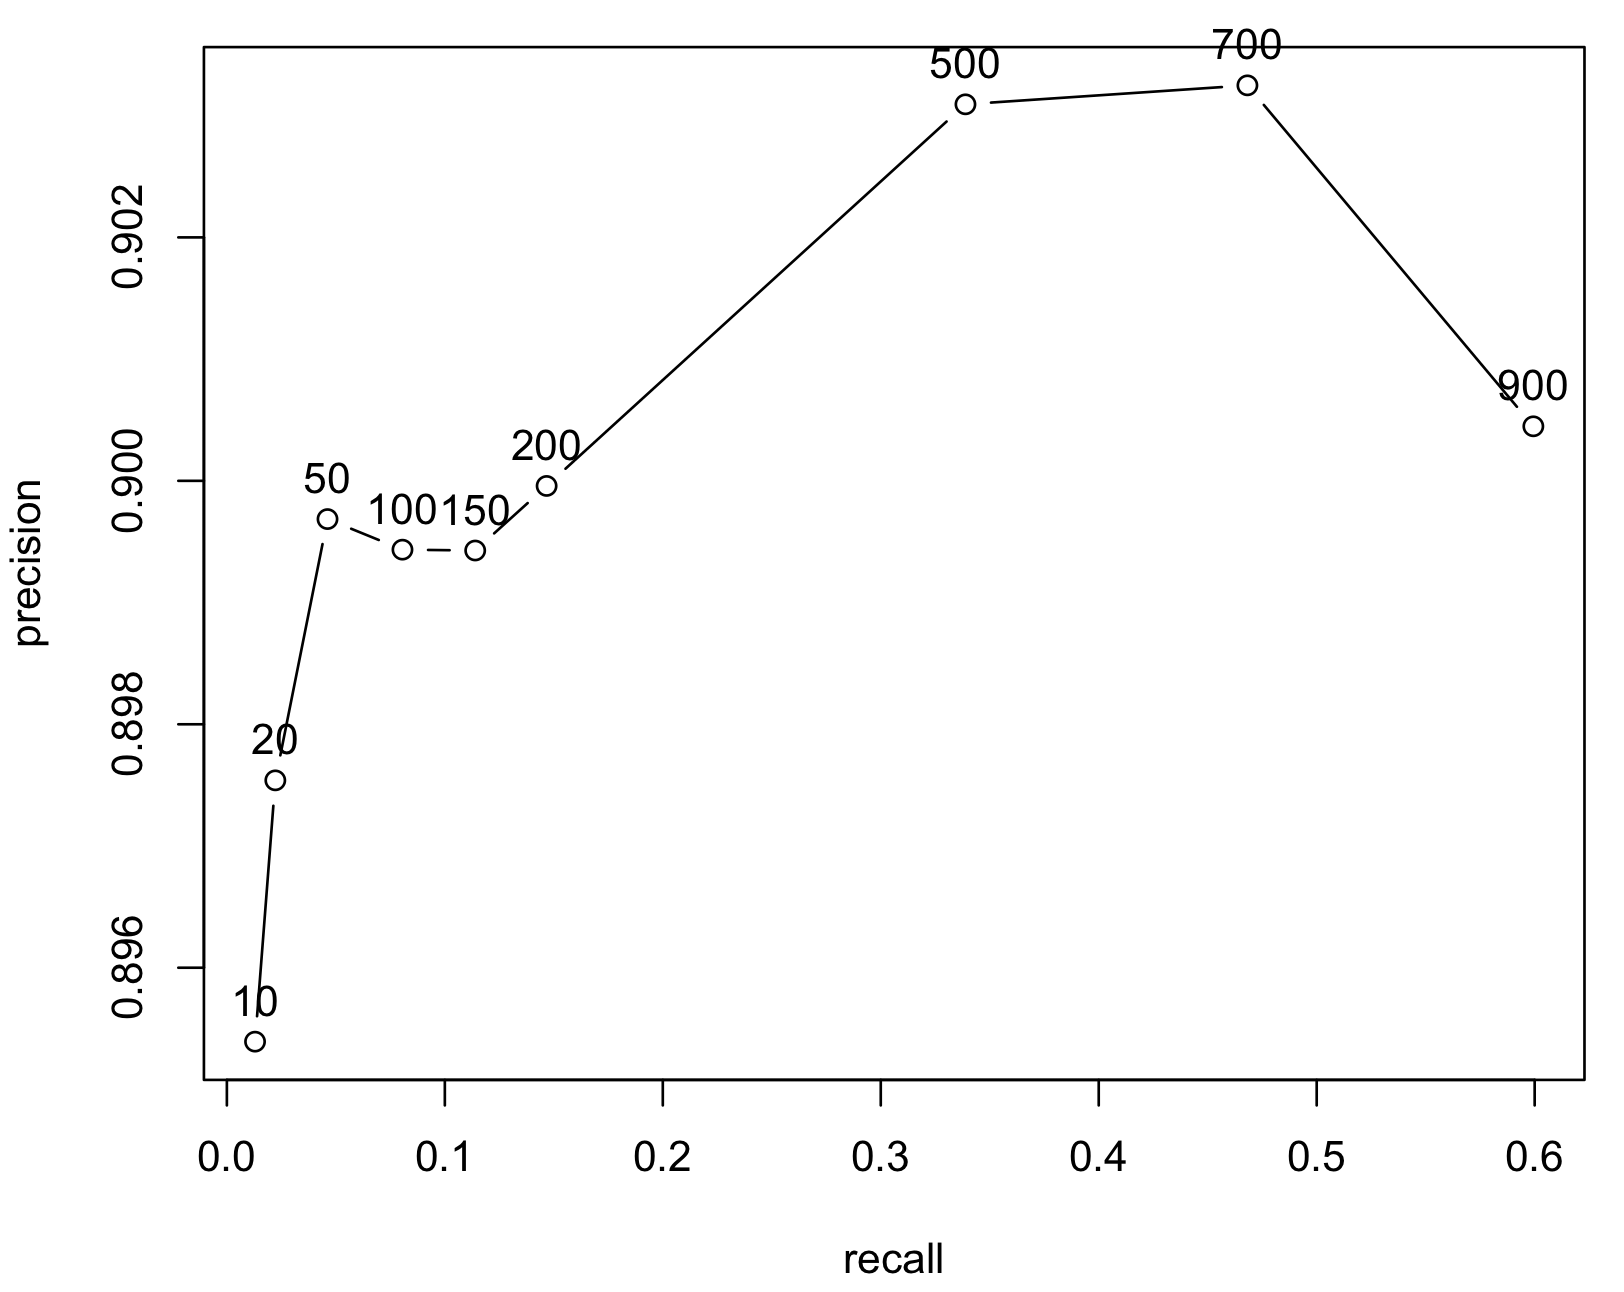
\includegraphics[width=0.6\textwidth]{gbhjj.png}
    \\\footnotesize Figure 1.6 : Precision vs Recall
\end{center}

The graph for TPR vs FPR could not be used to find an appropriate value for n. From the Precision vs Recall graph we can easily interpret that the best value for n was 50. This means that the best performance of our model was when the value for n was taken as 50.



    
\end{enumerate}

\newpage
\item\textbf{Problem 2}
\\
In this exercise, we consider the following ratings table between five users and six items.

\begin{center}
    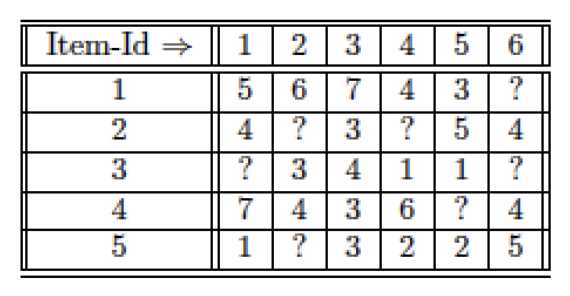
\includegraphics[height=0.2\textwidth]{hgjg.png}
    \\\footnotesize Table 2.1 : Ratings Table
\end{center}

\textbf{User Based Collaborative Filtering }
\\1. Look for users who share the same rating patterns with the active user (the user whom the prediction is for).
\\2. Use the ratings from those like-minded users found in step 1 to calculate a prediction for the active user.

\textbf{Item Based Collaborative Filtering }
\\1. Build an item-item matrix determining relationships between pairs of items.
\\2. Infer the tastes of the current user by examining the matrix and matching that user's data.

\begin{enumerate}
    \item We predicted the values of unspecified ratings of user 2 using user-based collaborative filtering. We used the Pearson correlation with mean-centering to normalize the data before predicting the ratings. While using this method we found that User 2 was highly similar to User 4 and User 5.
    \\The rating for Item 2 was found to be \textbf{4.08} and for Item 4 was found to be \textbf{3.84}.
    
    \item We predicted the values of unspecified ratings of user 2 using item-based collaborative filtering algorithms. We used the adjusted cosine similarity to normalize the data before predicting the ratings. While using this method we found that Item 2 was highly similar to Item 3 and Item 5.
    \\The rating for Item 2 was found to be \textbf{3.99} and for Item 4 was found to be \textbf{3.98}.
\end{enumerate}


The ratings predicted by both the methods gave similar ratings for the items. We cannot really differentiate between the performance of the two methods using this data set.
\newpage

\item \textbf{Problem 3}
\\
In this exercise, we were asked to examine the Boston Housing Data available in the ElemStatLearn package. The variables in the data set were as follows:
\\
\\CRIM per capita crime rate by town
\\ZN proportion of residential land zoned for lots over 25,000 sq.ft.
\\INDUS proportion of non-retail business acres per town
\\CHAS Charles River dummy variable (= 1 if tract bounds river; 0 otherwise)
\\NOX nitric oxides concentration (parts per 10 million)
\\RM average number of rooms per dwelling
\\AGE proportion of owner-occupied units built prior to 1940
\\DIS weighted distances to five Boston employment centres
\\RAD index of accessibility to radial highways
\\TAX full-value property-tax rate per \$ 10,000
\\PTRATIO pupil-teacher ratio by town
\\B 1000(Bk - 0.63)\^2  where Bk is the proportion of blacks by town
\\LSTAT lower status of the population
\\MEDV Median value of owner-occupied homes in \$ 1000's

\begin{enumerate}
    \item We visualized the data using histograms of the different variables in the data set. Using the inference from the histograms we transformed the data into a binary incidence matrix.
    \\We applied an ordered cut to the data by choosing the split after visualizing it using the following histograms and categorizing them into  low and high.
\begin{center}
    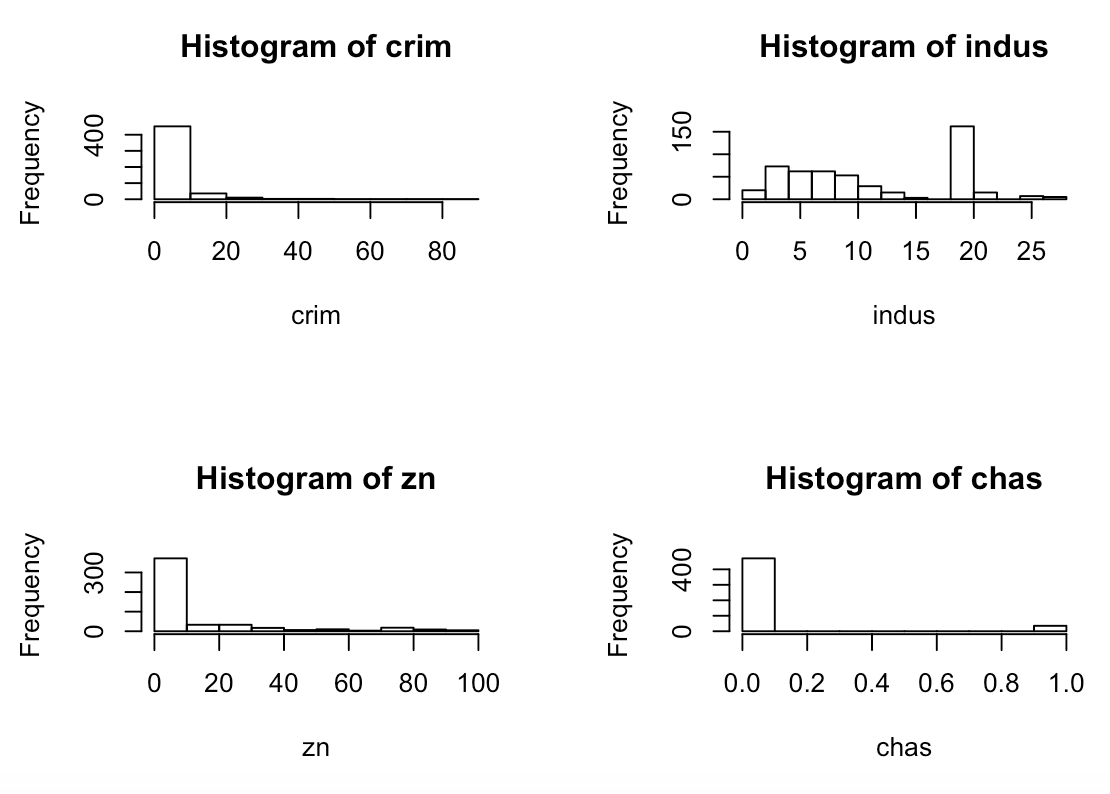
\includegraphics[height=0.5\textwidth]{s1_1.png}
    \\\footnotesize Figure 3.1 : Histograms for CRIM, ZN, INDUS, CHAS 

    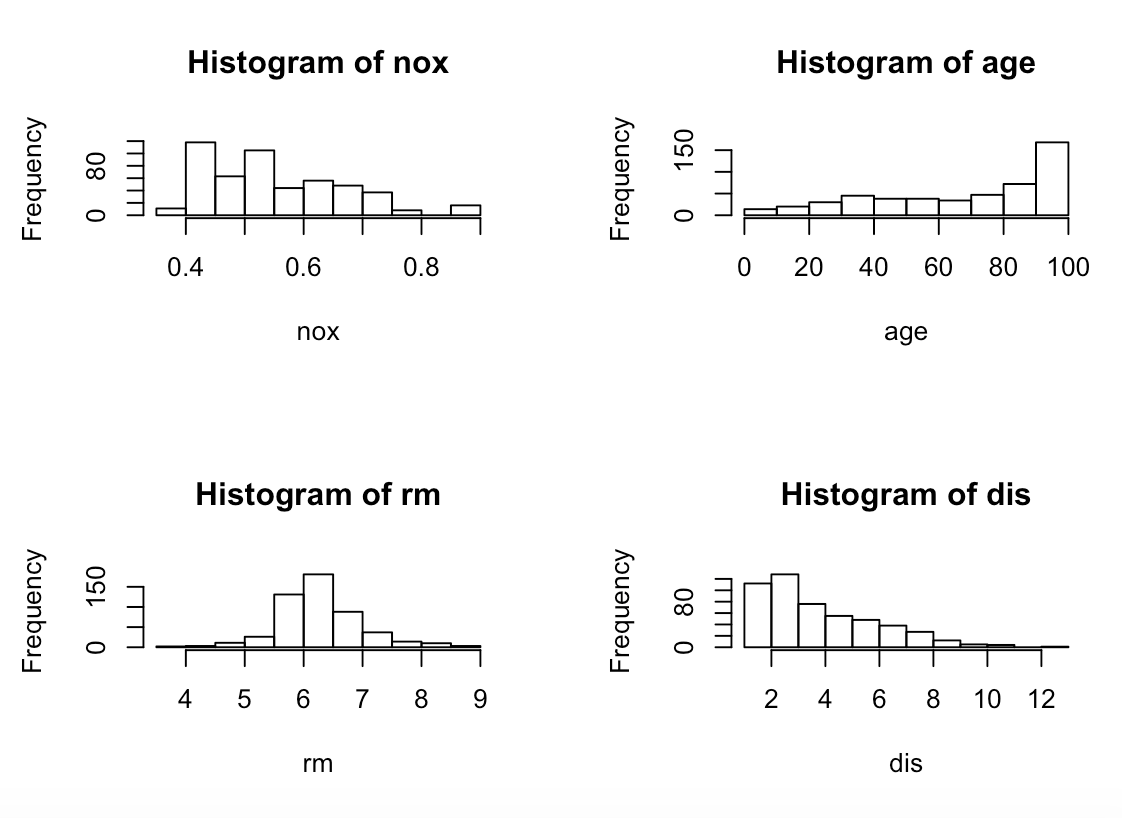
\includegraphics[height=0.5\textwidth]{s1_2.png}
    \\\footnotesize Figure 3.2 : Histograms for NOX, RM, AGE, DIS
    
    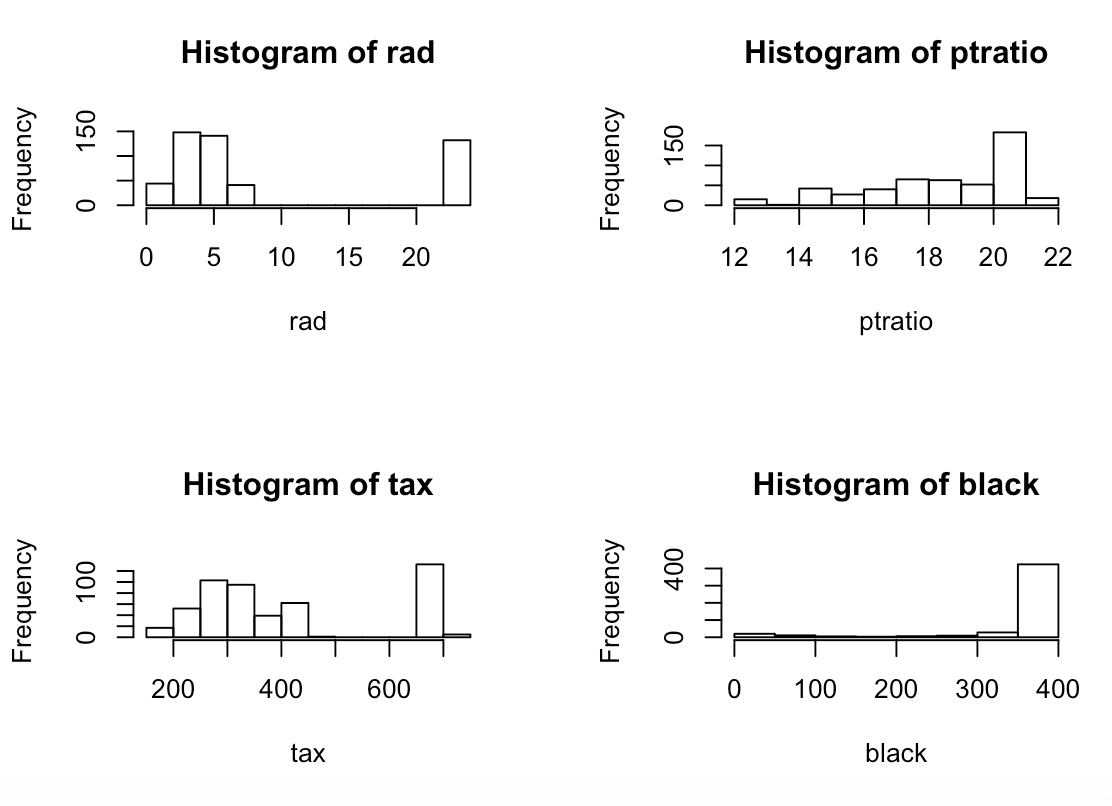
\includegraphics[height=0.5\textwidth]{s1_3.png}
    \\\footnotesize Figure 3.3 : Histograms for RAD, TAX, PTRATIO, BLACK
    
     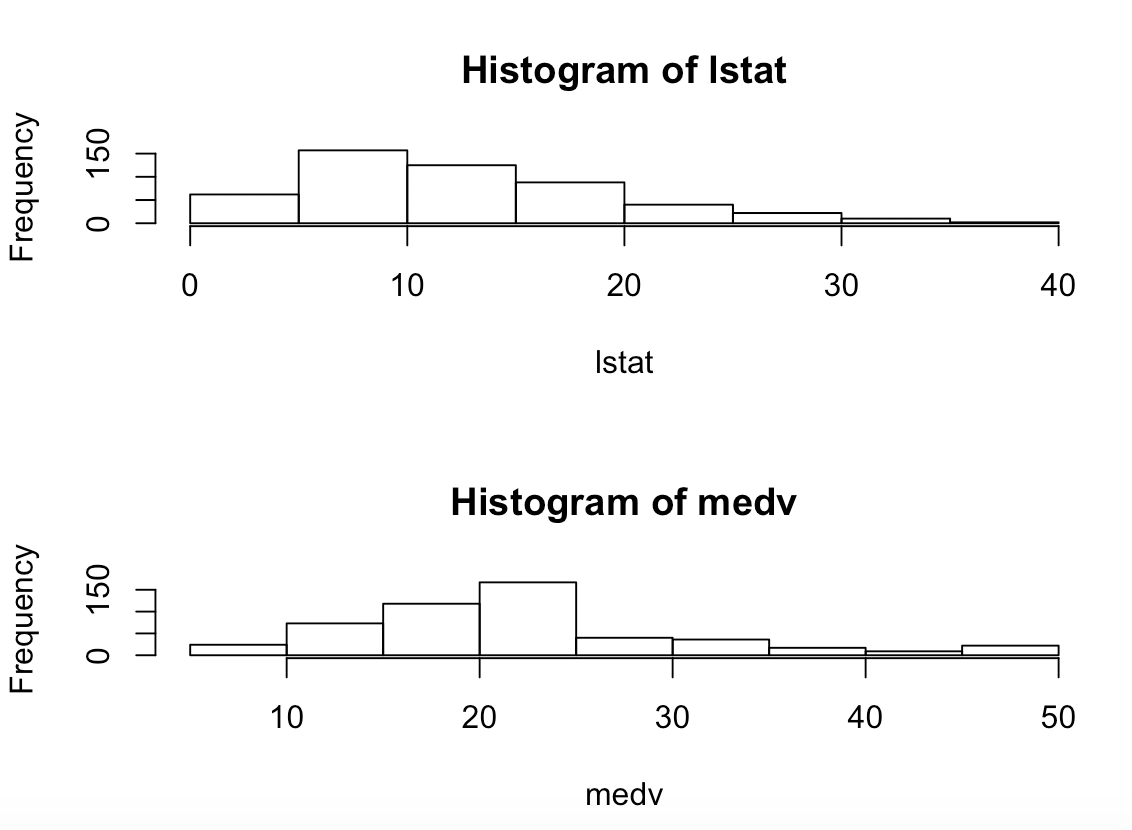
\includegraphics[height=0.5\textwidth]{s1_4.png}
    \\\footnotesize Figure 3.4 : Histograms for LSTAT, MEDV
\end{center}
    
    \item We visualized the data using the itemFrequencyPlot in the “arules” package. The parameter values for \textbf{support} was taken as \textbf{0.02} and for \textbf{confidence} as \textbf{0.8}.
    \begin{center}
    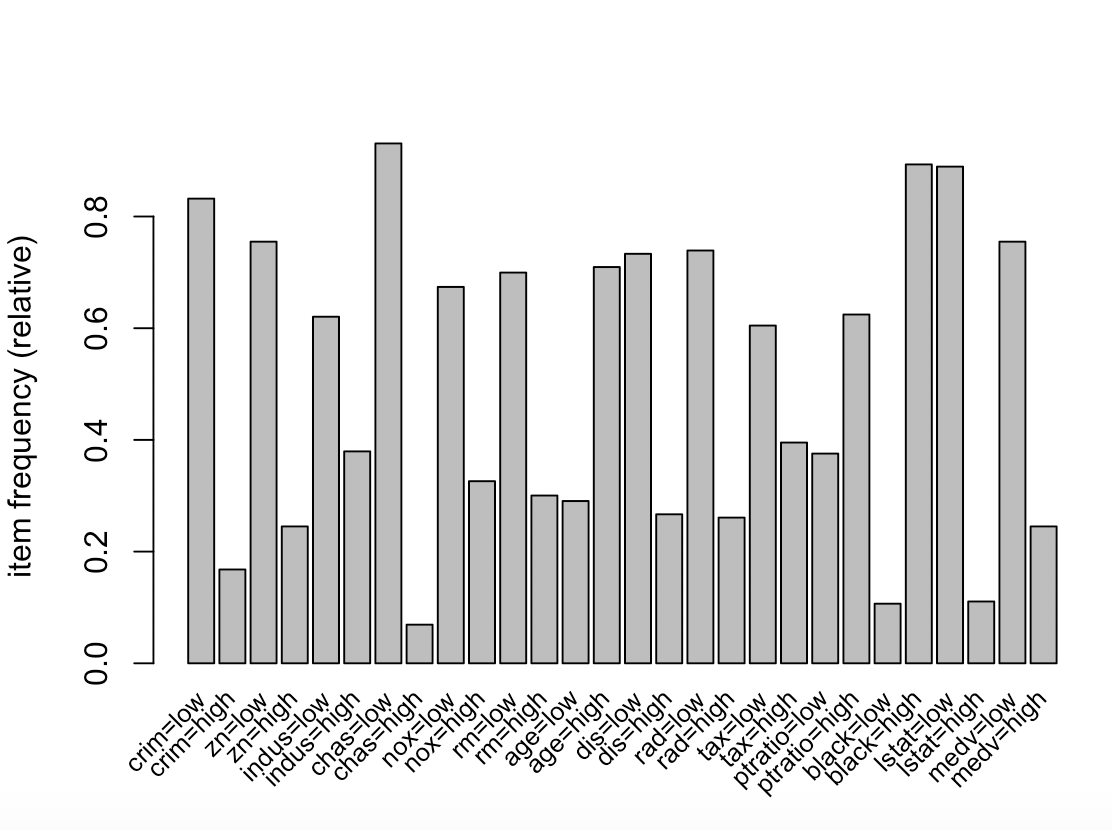
\includegraphics[height=0.5\textwidth]{s1_5.png}
    \\\footnotesize Figure 3.5 : itemFrequencyPlot 
   \end{center}
    With the above parameter values, we ended up with 804,413 rules.
    
    \item The  rules for the student interested in a low crime area as close to the city as possible (as measured by “dis”) can be  found by setting the antecedent as low crime and consequent as low distance. Lift is used to measure the ratio of confidence to support of the antecedent and consequent. We took lift to be greater than 1.2 to easily narrow down the rules.
    \\ We looked at the top 10 rules with the highest lift.
    \begin{center}
    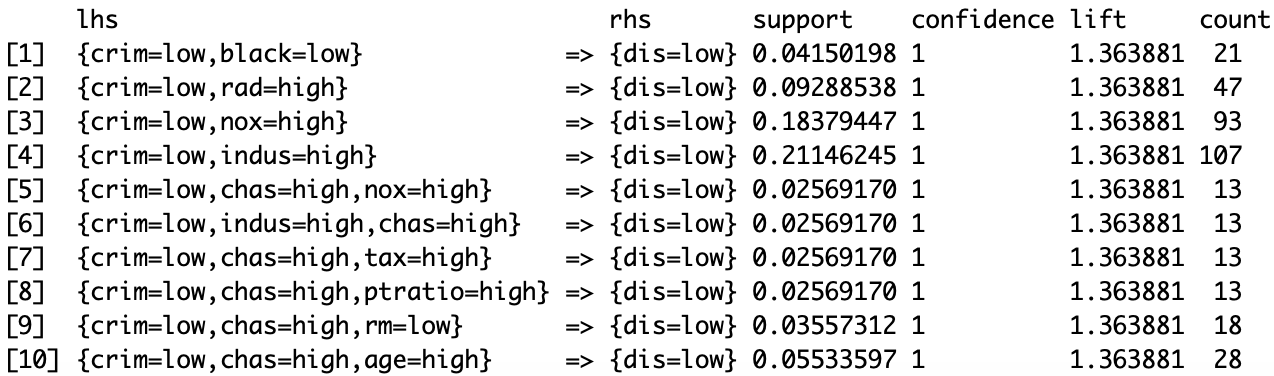
\includegraphics[width=0.6\textwidth]{sssshhhh.png}
    \\\footnotesize Figure 3.6 : Association rules for Crime=Low to Dis=Low 
\end{center}
    Through the above rules, we can advise that the areas with low black population, high rad high nox or high indus along with a low crime rate tend to have distances also as low.
    
    \item The  rules for the family interested in low pupil-teacher ratio can be  found by setting the consequent as low ptratio. Lift is used to measure the ratio of confidence to support of the antecedent and consequent. We took lift to be greater than 1.5 to easily narrow down the rules.
    \\ We looked at the top 10 rules with the highest lift.
    \begin{center}
    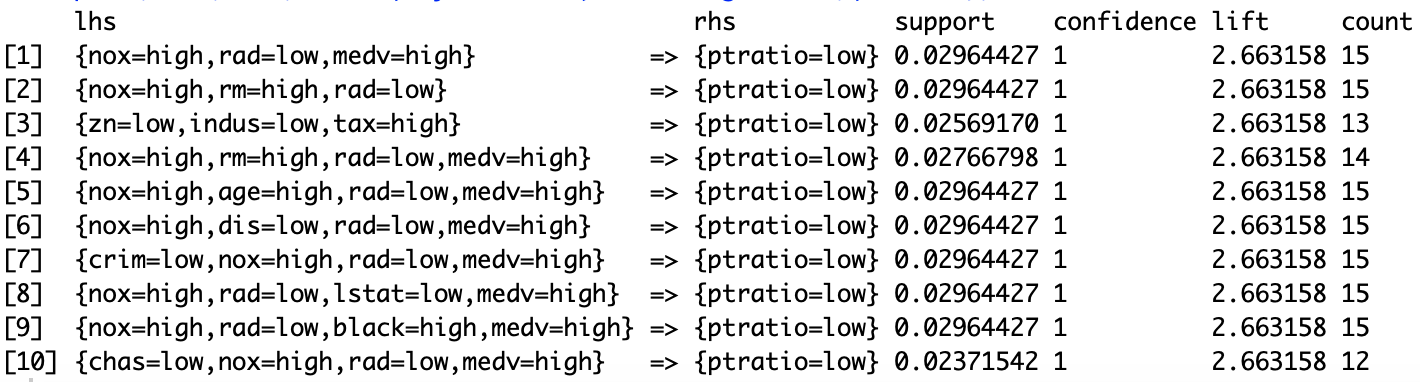
\includegraphics[width=0.6\textwidth]{sshhsshh.png}
    \\\footnotesize Figure 3.7 : Association rules for Ptratio=Low 
\end{center}
    Through the above rules, we can infer that a low pupil-teacher ratio depends highly on the nox being high, rad being low and medv being high. It also depends on rm being high and zn being low.
    
    
    \item We used a linear regression model to find characteristics of areas  with low pupil-teacher ratio. We ended up the following coefficients for the various attributes.
    \begin{center}
    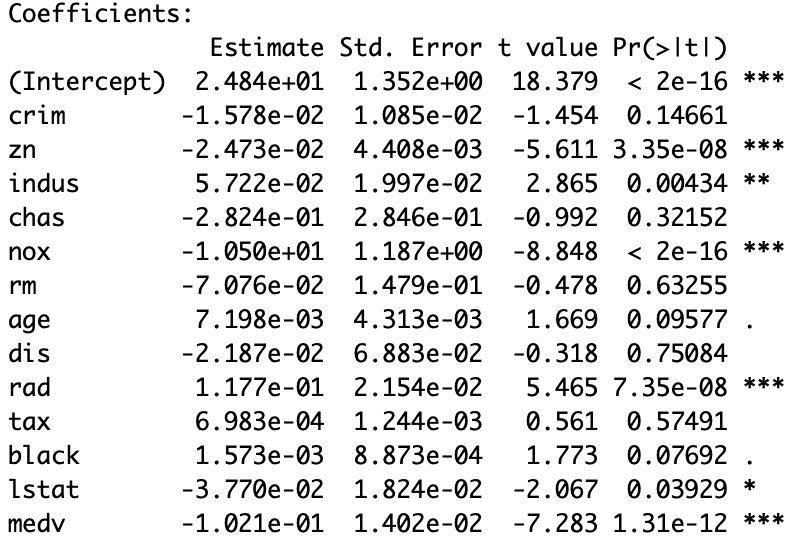
\includegraphics[width=0.6\textwidth]{shhshh.png}
    \\\footnotesize Figure 3.8 :Linear Model for Ptratio
\end{center}
    The results we obtained from the regression model are somewhat comparable to the association rules obtained earlier. It suggests the same variables
    to be significant which were actually involved in the top rules in the part (d). Linear regression gives an easier interpretation than association rules as association rules gives a broader look at the variables whereas linear regression gives us the real variable importance.
    \\Regression would be more suitable when we are trying to find out if the value of a pupil-teacher ratio would be low or high given some prior information about the area. Association models would be preferred when we know what kind of a value we want for the pupil-teacher ratio. It would be more accurate in telling us what kind of an area should we be searching for.
\end{enumerate}

\newpage
\item\textbf{Problem 4} 
\\
In this exercise, we were asked to cluster the demographic data from the following table using a classification tree.
\begin{center}
    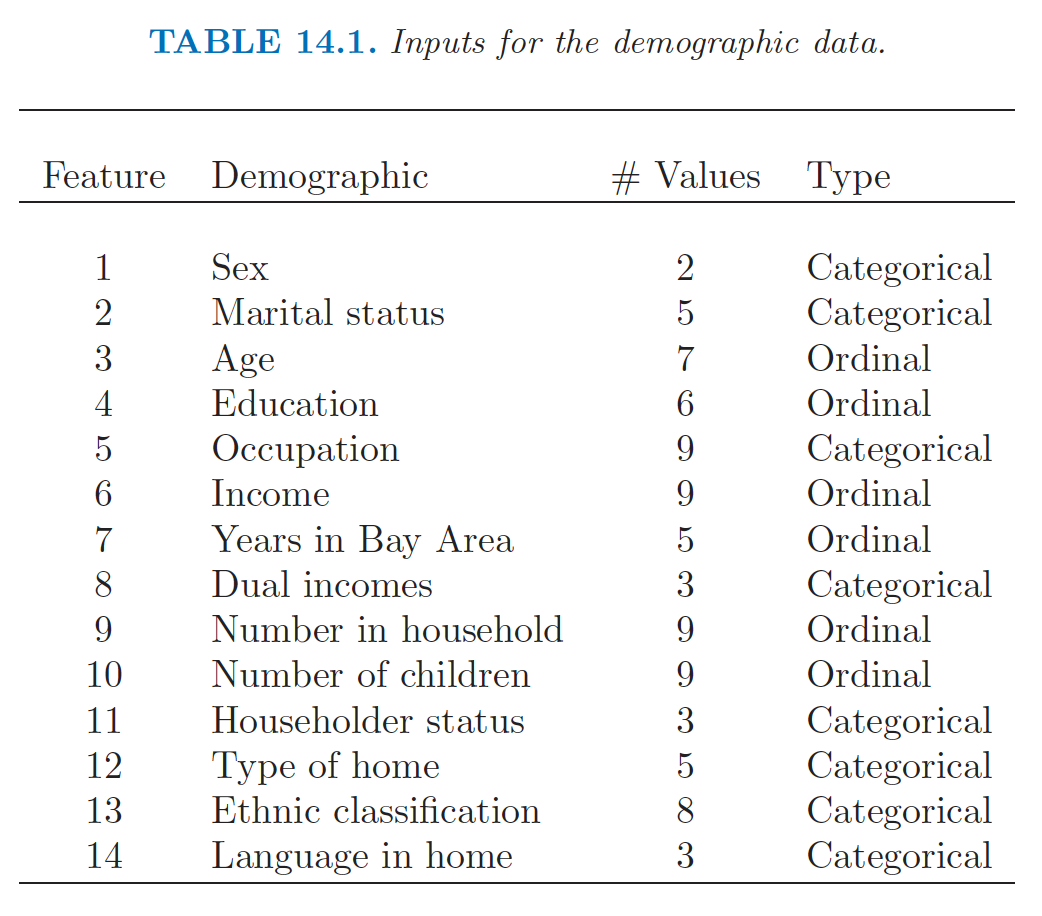
\includegraphics[height=0.4\textwidth]{sshhs.png}
    \\\footnotesize Table 4.1 : Demographic Data 
\end{center}

We used the marketing data from the ElemStatLearn for this exercise. We used the original data set and set a target variable for it as 1. We used the same data set to create a reference sample as the same size of the original data and give it a response variable with value of 0.

\\We then built a classification tree to the training sample (class 1) and the reference sample (class 0). We got the following tree from our model.

\begin{center}
    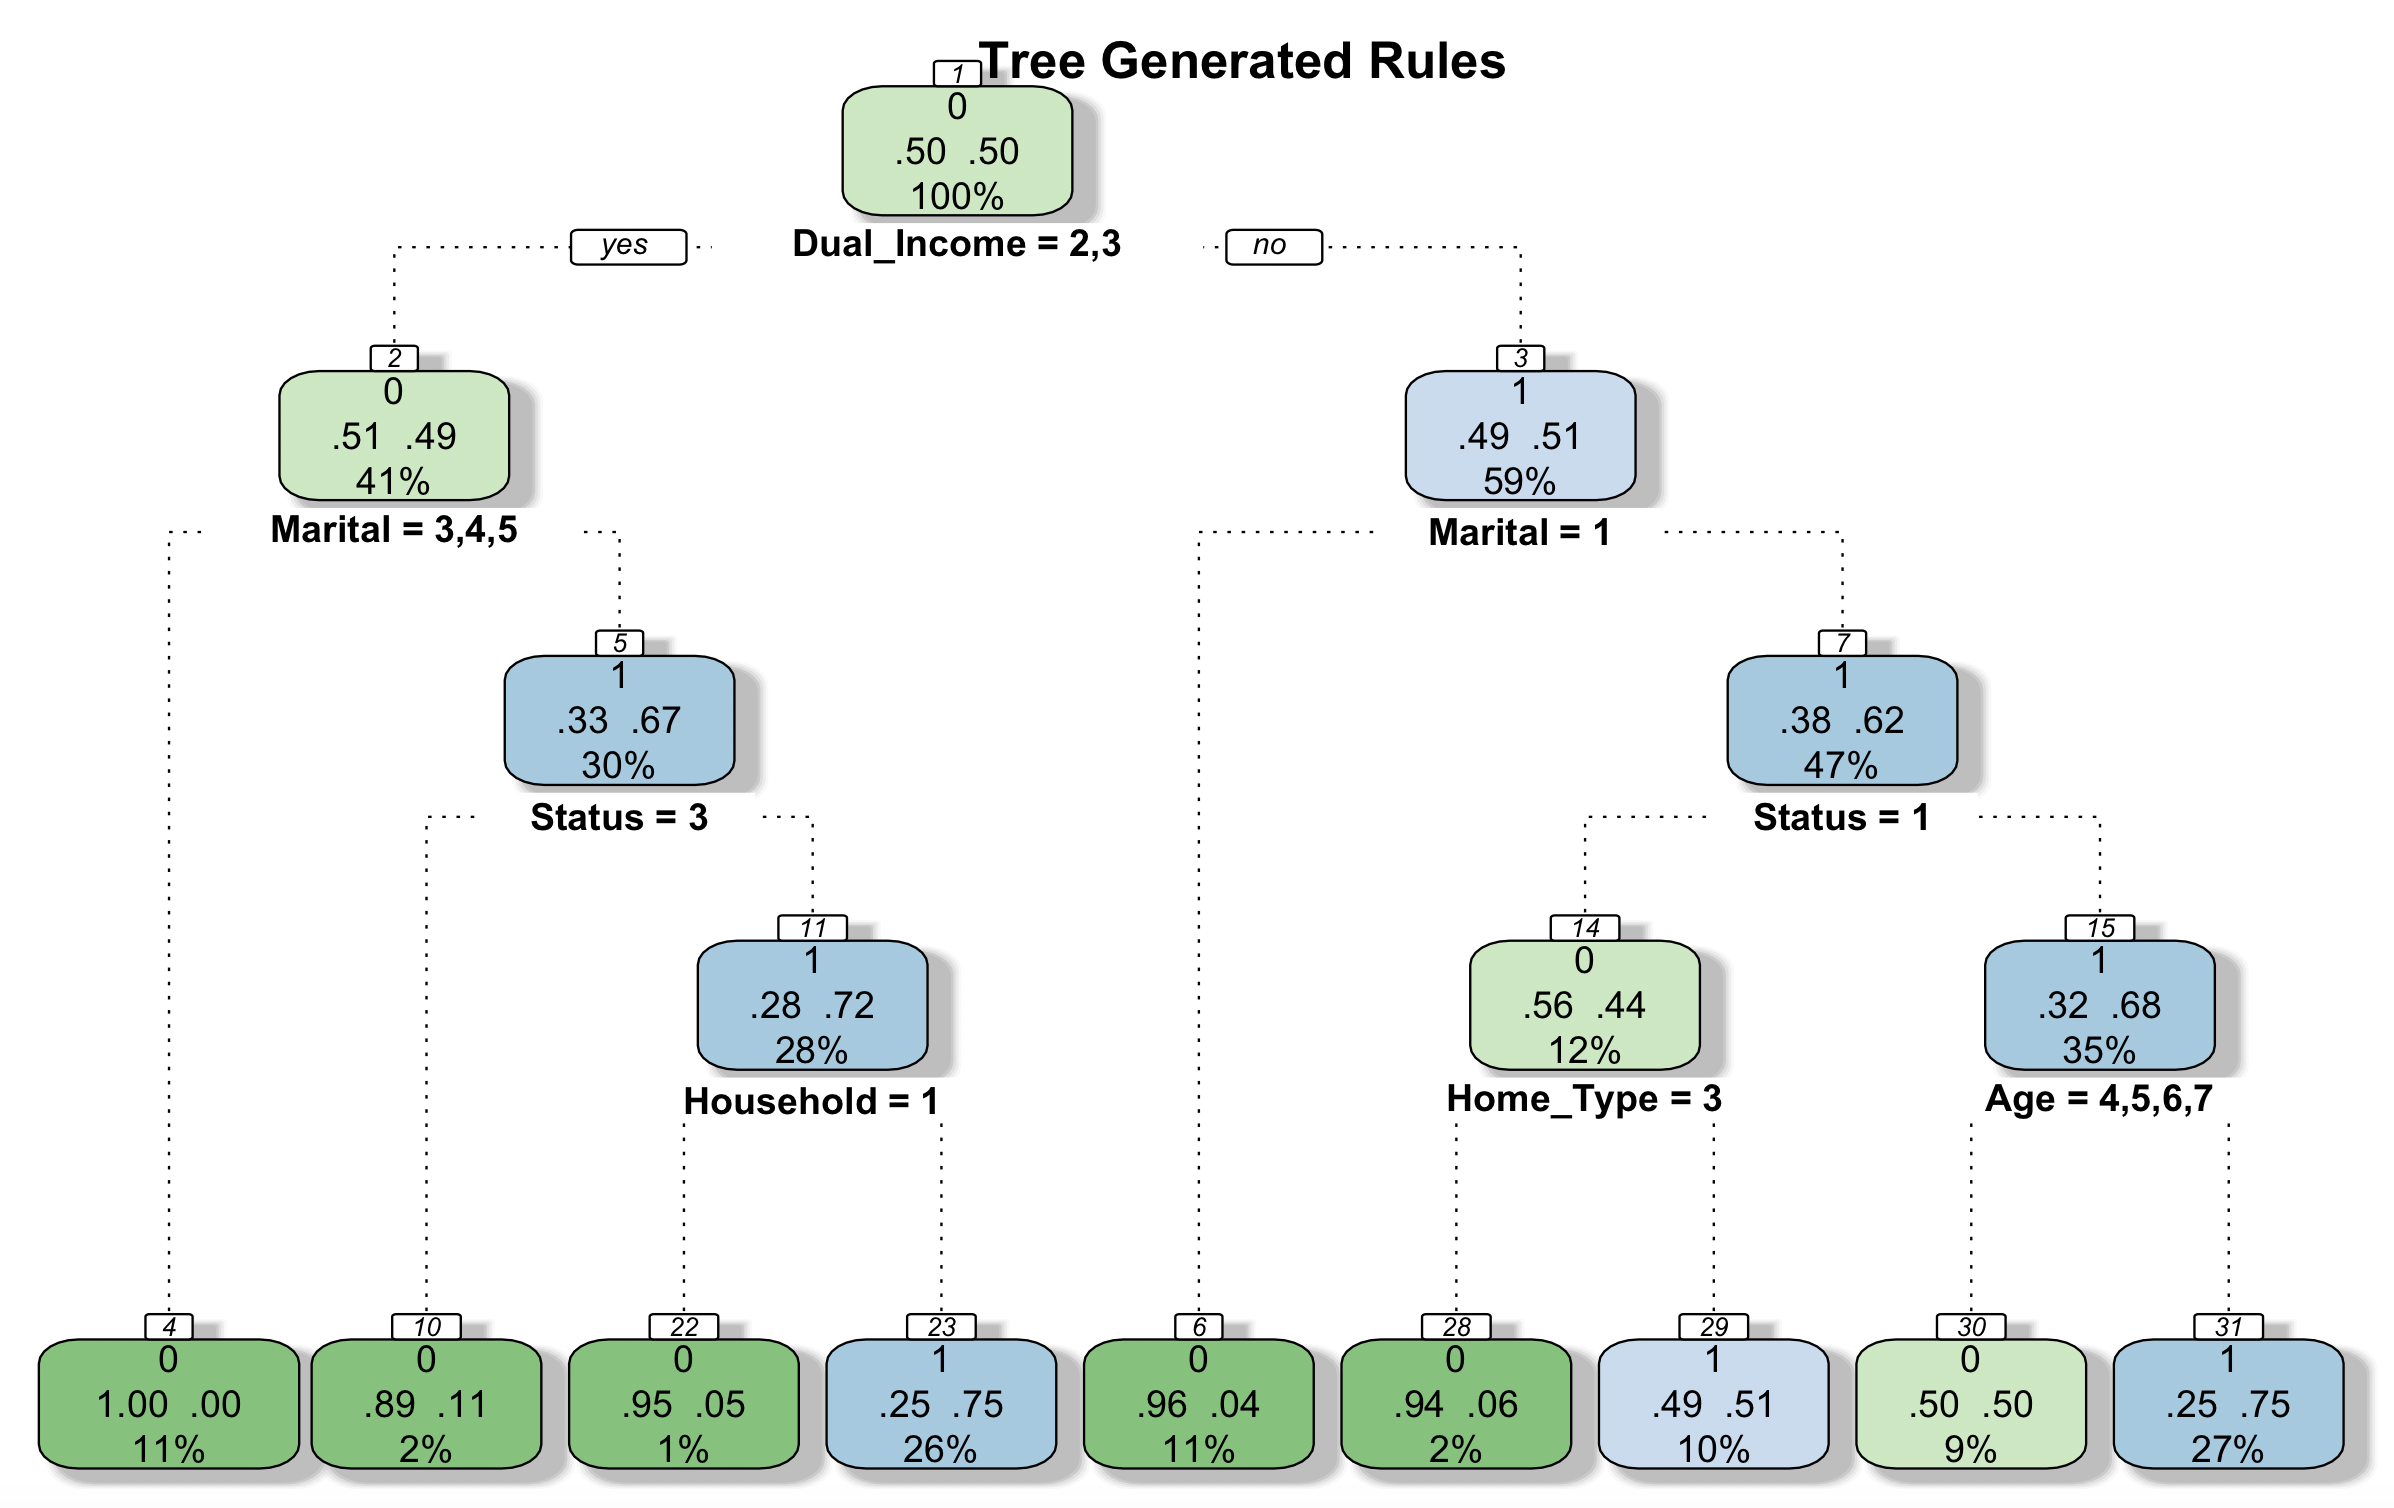
\includegraphics[height=0.5\textwidth]{fghf.png}
    \\\footnotesize Figure 4.1 : Tree Generated Rules 
\end{center}

There were two terminal nodes having highest estimated class 1 probability with a data percentage of 27 and estimated class 1 probability of 0.75. 

\\The first node had the following characteristics : Dual Income - Yes or No, Marital - Married or Living together, Status - Not living with parents and Persons living in household greater than 1.

\\The second node had the following characteristics : Dual Income - Not married, Marital - Not married, Status - Not Own and Age between 14-31.

\end{enumerate}
\end{document}